\documentclass[tikz]{standalone}
%
%------------------------- formatting --------------------------%
% fonts
\usepackage{textcomp}
% set font shape helvetica
\usepackage[scaled=0.92]{helvet}
\renewcommand{\familydefault}{\sfdefault}
%
\usetikzlibrary{calc, arrows.meta}
\usepackage{ifthen}
%
\newcommand{\PicLab}{}
%
\newlength{\PSep}
\newlength{\YOffSet}
\newlength{\tmp}
\newlength{\tmpp}
\newlength{\PicWidth}
%
\begin{document}
	%	
	\setlength{\PSep}{0.3ex}
	\setlength{\PicWidth}{6cm}
	%	
	\normalsize % font size
	%
	\begin{tikzpicture}[Label/.style={font=\bfseries, inner sep=0ex, xshift=1ex, anchor=west}]
		%
		% HO =================================================
		%
		% Rad53 --------------------------------------
		\path (0,0) node[inner sep=0ex] (Rad53) {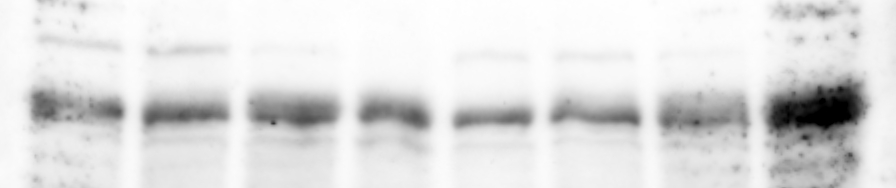
\includegraphics[width=\PicWidth]{Rad53_HO.jpg}};
		% frame
		\draw (Rad53.north west) rectangle (Rad53.south east);
		% label
		\draw (Rad53.east) node[Label] (Rad53Label) {$\alpha$-Rad53};
		% %---------------------------- grid -----------------------------%
		% \renewcommand{\PicLab}{Rad53}
		% % x
		% \foreach \x in {0,10,...,100}{
		% 	\draw[red, opacity=0.5] ($(\PicLab.north west)!\x/100!(\PicLab.north east)$) node[anchor=south,font={\tiny}] {\x} -- ($(\PicLab.south west)!\x/100!(\PicLab.south east)$);
		% }
		% \foreach \x in {5,15,...,95}{
		% 	\draw[red, opacity=0.25] ($(\PicLab.north west)!\x/100!(\PicLab.north east)$) -- ($(\PicLab.south west)!\x/100!(\PicLab.south east)$);
		% }
		% % y
		% \foreach \y in {0,10,...,100}{
		% 	\draw[red, opacity=0.5] ($(\PicLab.north west)!\y/100!(\PicLab.south west)$) node[anchor=east,font={\tiny}] {\y} -- ($(\PicLab.north east)!\y/100!(\PicLab.south east)$);
		% }
		% \foreach \y in {5,15,...,95}{
		% 	\draw[red, opacity=0.25] ($(\PicLab.north west)!\y/100!(\PicLab.south west)$) -- ($(\PicLab.north east)!\y/100!(\PicLab.south east)$);
		% }
		%--------------------------- labels ----------------------------%
		\begin{scope}[every node/.style={inner sep=0.5ex}]
			% 
			% time
			\pgfmathsetmacro{\Start}{0.095}
			\pgfmathsetmacro{\Sep}{0.117}
			\path (Rad53.north east) node[anchor=south west] (L) {Time (h)\strut};
			\foreach[count=\i from 1] \x in {0, 1, 2, 4, 0, 1, 2, 4}{
				\pgfmathsetmacro{\y}{\Start+(\i-1)*\Sep}
				% alternating offset
				\pgfmathtruncatemacro{\rest}{mod(\i,2)}
				\ifthenelse{\rest = 0}{\setlength{\YOffSet}{0ex}}{\setlength{\YOffSet}{0ex}}
				\path ($(Rad53.north west)!\y!(Rad53.north east)$) coordinate (x);
				\path ($(x|-L.south)+(0,\YOffSet)$) node[anchor=south] (L\i) {\x\strut};
			}
			%
			% fun30
			\setlength{\tmp}{0.25ex}
			\path (L.north west) node[anchor=south west] (S) {\strut};
			\path ($(L.north)!0.5!(S.south)$) coordinate (y);	
			\draw ($(L1.west|-y)+(-\tmp,0)$) -- ($(L4.east|-y)+(\tmp,0)$) node[midway] (x) {};
			\path (x|-S) node {WT};
			\draw ($(L5.west|-y)+(-\tmp,0)$) -- ($(L8.east|-y)+(\tmp,0)$) node[midway] (x) {};
			\path (x|-S) node {\textit{fun30$\Delta$}};
			%
			% HO
			\setlength{\tmp}{0.25ex}
			\path (S.north west) node[anchor=south west] (D) {\strut};
			\path ($(S.north)!0.5!(D.south)$) coordinate (y);	
			\draw ($(L1.west|-y)+(-\tmp,0)$) -- ($(L8.east|-y)+(\tmp,0)$) node[midway] (x) {};
			\path (x|-D) node {HO-induced DSB};
			%
			% kDa
			\draw ($(Rad53.north west)!0.17!(Rad53.south west)-(1\PSep,0)$) -- ++(-2ex, 0ex) node[anchor=east] {150 kDa};
			\draw ($(Rad53.north west)!0.63!(Rad53.south west)-(1\PSep,0)$) -- ++(-2ex, 0ex) node[anchor=east] {100 kDa};
			\draw ($(Rad53.north west)!0.95!(Rad53.south west)-(1\PSep,0)$) -- ++(-2ex, 0ex) node[anchor=east] {75 kDa};
			%
		\end{scope}
		%
		% Pgk1 -----------------------------------
		\path (Rad53.south) ++(0,-1.5ex) node[inner sep=0ex, anchor=north] (Pgk1) {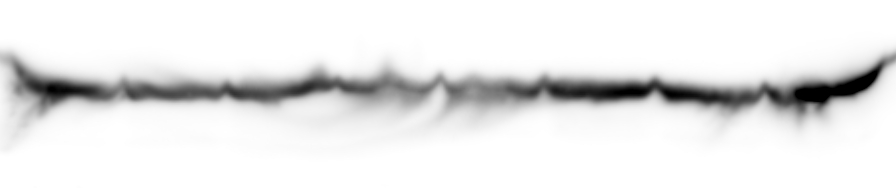
\includegraphics[width=\PicWidth]{Pgk1_HO.jpg}};
		% frame
		\draw (Pgk1.north west) rectangle (Pgk1.south east);
		% label
		\draw (Pgk1.east) node[Label] {$\alpha$-Pgk1};
		% %---------------------------- grid -----------------------------%
		% \renewcommand{\PicLab}{Pgk1}
		% % x
		% \foreach \x in {0,10,...,100}{
		% 	\draw[red, opacity=0.5] ($(\PicLab.north west)!\x/100!(\PicLab.north east)$) node[anchor=south,font={\tiny}] {\x} -- ($(\PicLab.south west)!\x/100!(\PicLab.south east)$);
		% }
		% \foreach \x in {5,15,...,95}{
		% 	\draw[red, opacity=0.25] ($(\PicLab.north west)!\x/100!(\PicLab.north east)$) -- ($(\PicLab.south west)!\x/100!(\PicLab.south east)$);
		% }
		% % y
		% \foreach \y in {0,10,...,100}{
		% 	\draw[red, opacity=0.5] ($(\PicLab.north west)!\y/100!(\PicLab.south west)$) node[anchor=east,font={\tiny}] {\y} -- ($(\PicLab.north east)!\y/100!(\PicLab.south east)$);
		% }
		% \foreach \y in {5,15,...,95}{
		% 	\draw[red, opacity=0.25] ($(\PicLab.north west)!\y/100!(\PicLab.south west)$) -- ($(\PicLab.north east)!\y/100!(\PicLab.south east)$);
		% }
		%--------------------------- labels ----------------------------%
		\begin{scope}[every node/.style={inner sep=0.5ex}]
			% 
			% kDa
			\draw ($(Pgk1.north west)!0.22!(Pgk1.south west)-(1\PSep,0)$) -- ++(-2ex, 0ex) node[anchor=east] {50 kDa};
			\draw ($(Pgk1.north west)!0.85!(Pgk1.south west)-(1\PSep,0)$) -- ++(-2ex, 0ex) node[anchor=east] {37 kDa};
			%
		\end{scope}
		%
		%
	\end{tikzpicture}
	%
\end{document}